\begin{table}[!t]
\centering
\caption{Métricas das previsões externas da validação aninhada (\%)}
\label{tab:results}
\footnotesize
\setlength{\tabcolsep}{2.6pt}
\begin{tabular}{@{}llrrrrrrr@{}}
\toprule
Cenário & Família & BA & Sens. & Esp. & Prec. & \(F_1\) & AUC & AP \\
\midrule
\multirow{4}{*}{\textsc{Clinico}} & Maioria & 50,00 & 0,00 & 100,00 & 0,00 & 0,00 & 50,00 & 42,38 \\
 & Árvore & \textbf{91,94} & 87,50 & 96,38 & 94,68 & 90,95 & 92,29 & 91,38 \\
 & Logística & 91,90 & 87,40 & 96,40 & 94,70 & 90,90 & 94,02 & 93,70 \\
 & Floresta & 91,91 & 87,37 & 96,46 & 94,78 & 90,92 & 94,74 & 94,43 \\
\midrule
\multirow{4}{*}{\textsc{Fisio8}} & Maioria & 50,00 & 0,00 & 100,00 & 0,00 & 0,00 & 50,00 & 42,38 \\
 & Árvore & 60,91 & 54,32 & 67,50 & 55,14 & 54,73 & 63,68 & 56,00 \\
 & Logística & 61,64 & 55,51 & 67,78 & 55,89 & 55,70 & 65,64 & 56,67 \\
 & Floresta & \textbf{62,91} & 58,91 & 66,91 & 56,70 & 57,78 & 67,20 & 59,55 \\
\midrule
\multirow{4}{*}{\textsc{Strict4}} & Maioria & 50,00 & 0,00 & 100,00 & 0,00 & 0,00 & 50,00 & 42,38 \\
 & Árvore & 59,32 & 35,82 & 82,81 & 60,52 & 45,00 & 61,53 & 54,37 \\
 & Logística & \textbf{59,74} & 52,03 & 67,45 & 54,03 & 53,01 & 63,66 & 55,78 \\
 & Floresta & 59,67 & 49,61 & 69,73 & 54,65 & 52,01 & 64,35 & 57,46 \\
\bottomrule

\end{tabular}
\par\smallskip
\raggedright\scriptsize Sens.\ = sensibilidade; Esp.\ = especificidade; AUC = área sob a curva ROC. Maioria é o baseline simples. Em negrito, a maior BA de cada cenário. Precisão e \(F_1\) da maioria valem zero porque ela não prevê positivos.
\end{table}

\subsection{Comparação entre cenários e famílias}
A Tabela~\ref{tab:results} reúne as previsões externas dos \nDev{} registros de desenvolvimento. Em \clinico{}, árvore, logística e floresta ficam a \clinBAspread{} ponto percentual uma da outra em BA, um empate prático. Pelo critério fixado antes da execução, a árvore tem a maior BA (\vClinArvBA\%), com sensibilidade de \vClinArvSens\% e especificidade de \vClinArvEsp\%. A floresta ordena melhor as probabilidades (ROC-AUC de \vClinFloAUC\% contra \vClinArvAUC\% da árvore), o que importa se o limiar for ajustado. O modelo final da árvore usa \finalClinParams{} e \finalClinImput{}; com profundidade dois, ele equivale a uma regra sobre poucos atributos.

Retirar os achados de exame derruba o desempenho: a melhor BA cai \ganhoClinFisio{} pontos, para \vFisioFloBA\% (\bestFisio{} em \fisio{}). Retirar também os sinais vitais tira mais \ganhoFisioStrict{} pontos, para \vStrictLogBA\% (\bestStrict{} em \strict{}). Nos dois cenários de sensibilidade, os modelos superam o baseline, mas discriminam pouco.

\begin{table}[!t]
\centering
\caption{Matrizes de confusão das previsões externas}
\label{tab:confusion}
\footnotesize
\begin{tabular}{@{}lrrrr@{}}
\toprule
& \multicolumn{2}{c}{\clinico{} (árvore)} & \multicolumn{2}{c}{\fisio{} (floresta)} \\
\cmidrule(lr){2-3}\cmidrule(l){4-5}
Rótulo & Normal & Anormal & Normal & Anormal \\
\midrule
Normal & \vClinArvTN & \vClinArvFP & \vFisioFloTN & \vFisioFloFP \\
Anormal & \vClinArvFN & \vClinArvTP & \vFisioFloFN & \vFisioFloTP \\
\bottomrule
\end{tabular}
\par\smallskip
\raggedright\scriptsize Linhas: rótulo registrado. Colunas: classe prevista.
\end{table}

\begin{figure*}[!t]
\centering
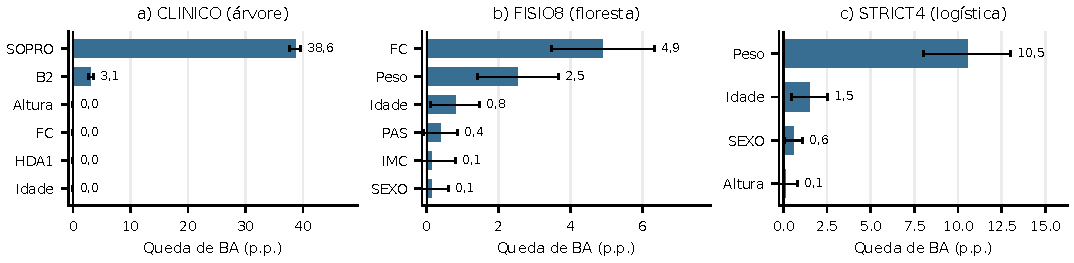
\includegraphics[width=\textwidth]{importancia.pdf}
\caption{Importância por permutação no modelo de maior BA de cada cenário: queda média de BA ao embaralhar o atributo no \textit{fold} externo (5 \textit{folds} $\times$ 3 repetições; barras de erro: desvio-padrão). Seis atributos de maior queda por painel.}
\label{fig:importance}
\end{figure*}

\subsection{De onde vem a informação}
A Fig.~\ref{fig:importance} mostra que, em \clinico{}, embaralhar SOPRO reduz a BA em \impClinSopro{} pontos e embaralhar B2, em \impClinBtwo{}; para os demais atributos a queda é nula, porque as árvores selecionadas só usam esses dois. O ganho de \clinico{} sobre \fisio{} vem, portanto, da ausculta. Isso é coerente com o fluxograma de investigação do material complementar, que parte justamente de sopro, B2 e pulsos \cite{guideline}. Sem o exame físico, a floresta de \fisio{} passa a depender da FC (\impFisioFC{} pontos) e do Peso (\impFisioPeso{}), e a logística de \strict{}, do Peso (\impStrictPeso{}). FC e Peso variam fortemente com a idade, e os anormais são mais novos; boa parte do sinal desses atributos parece refletir a idade e o crescimento, e não um achado cardíaco. Em \clinico{}, a FC perde a importância (\impClinFC{} ponto), porque o sopro já carrega a informação que ela trazia.

A diferença de idade entre as classes é compatível com o predomínio de cardiopatias congênitas, que costumam se manifestar e ser diagnosticadas nos primeiros meses de vida. Os números descrevem associação neste serviço e não estabelecem causa.

\subsection{Análise de erros}
A Tabela~\ref{tab:confusion} mostra que a árvore de \clinico{} deixa \vClinArvFN{} anormais como \textit{Normal}, \clinFNpctAnormal\% dos anormais. Todos esses falsos negativos (\errClinFNsemSopro\%) são registros sem sopro: o desenvolvimento tem \anormSemSopro{} anormais sem sopro (\anormSemSoproPct\% dos anormais), e o modelo reconhece poucos deles. Já \errClinFPcomSopro\% dos \vClinArvFP{} falsos positivos têm sopro; há \normComSopro{} crianças normais com sopro, o que é compatível com sopros inocentes, frequentes na infância. Em uma triagem, os dois erros têm custos diferentes: o falso positivo leva a um exame complementar desnecessário, enquanto o falso negativo pode adiar o diagnóstico de uma cardiopatia. Por isso a sensibilidade de \vClinArvSens\% é o número a melhorar, e o limiar de 0,5 não é o ponto de operação ideal para esse uso.

\begin{table}[!t]
\centering
\caption{BA no teste histórico (\%), avaliação secundária}
\label{tab:test}
\footnotesize
\begin{tabular}{@{}lrrr@{}}
\toprule
Cenário & Árvore & Logística & Floresta \\
\midrule
\textsc{Clinico} & 92,92 & 93,06 & 92,90 \\
\textsc{Fisio8} & 64,27 & 62,85 & 65,23 \\
\textsc{Strict4} & 61,53 & 60,33 & 61,46 \\
\bottomrule

\end{tabular}
\par\smallskip
\raggedright\scriptsize \nTest{} registros; o teste foi examinado em fases anteriores do projeto e não é intocado.
\end{table}

\subsection{Teste histórico}
Os modelos finais, aplicados uma vez aos \nTest{} registros do teste histórico (Tabela~\ref{tab:test}), mantêm a ordem entre cenários: \tClinArvBA\% de BA para a árvore de \clinico{}, \tFisioFloBA\% para a floresta de \fisio{} e \tStrictLogBA\% para a logística de \strict{}. Os valores ficam próximos dos da validação aninhada, o que indica estabilidade dentro da mesma coorte, mas não substitui uma validação externa.
